\documentclass[11pt]{article}

\usepackage{graphicx}
\usepackage[utf8]{inputenc}

\usepackage[left=1.2in,top=1.2in,right=1.2in,bottom=1.0in]{geometry} % Document margins

\title{\textbf{Toy DB Project Report \\ 
	Disk Storage Simulator \\
	Project No. 2 }}

\author{Rohit Kumar \\ 120050028 \\ rohit@cse.iitb.ac.in
		\and 
		Deependra Patel \\ 120050032 \\ pateldeependra06@gmail.com
		}

\date{\today}
\begin{document}

\maketitle

\section{Introduction}
\paragraph{}

This report talks about a strategic simulation of a disk system. The simulation includes an efficient arm movement strategy for processing the requests on a disk system, providing reliability, high performance through implementation of the \textbf{RAID-5} technology and caching unit for faster access. 

This disk-system is accessed during read and write requests randomly. The statistics related to various performance parameters are gathered and various conclusions and effect of the technologies used are displayed through graphs etc.
	
\section{Structure of the disk-system}
\paragraph{}

A main controller controls and executes all the functionalities provided. 

The main controller provides a mapping of page number to disk addresses. It has an access to a cache controller which manages the disk cache and interfaces between the disk-system and the main controller. The cache controller checks if the data is present in the cache and returns it. If not present, it passes the request to a disk controller which simulates the disk-system. The disk controller passes this request to a request buffer which in turn processes these requests using the elevator algorithm.

While processing the requests various logs and data relating to measure the performance parameters etc. are also being stored.

The details of the various data structures and algorithms used in these classes are described in the below section.

\section{Data Structures and Algorithm used for various classes}

\subsection{Main Controller \\ (mainController.cpp \& mainController.h)}
\paragraph{}
The main controller stores a mapping of page numbers of a particular file to the disk address. For implementing this functionality, the map data structure provided by the STL of c++ has been used. Whenever a read request for a particular page in particular file is made by the paged file module to this, it checks in the map if an address corresponding to this page is present in the map. If present, a read request is made to the cache controller, otherwise if there is no such mapping, it denotes that the page wasn't written in the disk earlier and it is an invalid request. In case of the request is invalid, it is dropped.

Whenever a write request is made, it is checked that the mapping is already present in the map or not. In case it is present, it implies that the file is already present and is being overwritten. In case if it is not present (implying writing for the first time), a new mapping is assigned to the page randomly from the set of available free addresses in the disk and this mapping is put in the map.

There might be a case when the file is being deleted from the disk. In such a case the mapping is no longer necessary and it is deleted from the map.

This main controller passes the requests to the cache controller for performing the operations.

\subsection{Cache Controller \\ (cacheController.cpp \& cacheController.h)}
\paragraph{}
Cache for disks is implemented in this class. We have implemented fully associative cache as miss penalty is huge for reading and writing data to the disks. On receiving the diskAddress to read and write from mainController, it checks whether the page is already present in the cache. If already found in cache, Page data is returned from there. If requested page is not found in cache, then new page is allocated to it and that page is brought from disk using diskController.

For page allocation, if any page is free that is allocated. If no free page found then page which is not dirty is allocated, if no such found then Least Recently Used(LRU) page is allocated after writing its contents to the disk.


An unordered map is used to keep mapping of disk address to corresponding page number in cache. Two boolean arrays of free pages and dirty pages is also kept. Whenever a page is written in cache, dirty flag is marked true. If any page marked dirty is to be removed from cache then its data has to be written back to disk. A linked list of pages is kept to store the allocated pages ordered by time. LRU is implemented on these pages by popping out first element on page allocation and pushing back the newly allocated page.


\subsection{Disk-System Controller \\ (diskController.cpp \& diskController.h)}
\paragraph{}
Disk Controller handles all the requests(read/write) made to the disk. The input disk address is first translated into corresponding disk and CHS(Cylinder Head Sector) format. As we are using RAID5, parity disk for that sector is also calculated. For calculating disk number, we are using Right Asynchronous RAID5 type as given below:


\begin{figure}[ht!]
\center
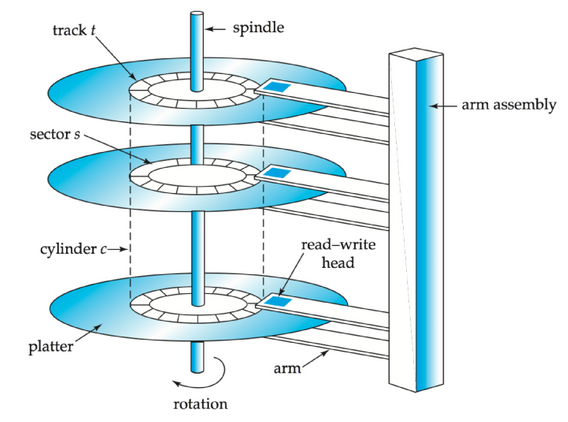
\includegraphics[scale = 0.70]{images/disk.png}
\caption{Design of the RAID-5 system and distribution of parity blocks}
\label{overflow}
\end{figure}

\subsubsection{Disk Number and CHS conversion}
In case of a RAID-5 system, the CHS conversion is complicated to normal conversion. In this scenario we have to take care of the parity block. The data block may need to be shifted in the next block to accommodate the parity block.


Let there be D disks are used in RAID5 (D+1 in total), each with each with N cylinders, M tracks/cylinder, and K sectors per track. Then the disk address of this sector can be calculated as :
\\
\begin{itemize}
\item d is the disk number. d  belongs to [ 0, 1, 2, …  D] 
\item c is the cylinder number. c belongs to [0, 1, 2, … N - 1] 
\item t is the head/track number. h belongs to [0, 1, 2, … M - 1] 
\item s is the sector number. s belongs to  [0, 1, 2, … K - 1] 
\item p is parity disk corresponding to a CHS 
\item a is address in that disk \\
\end{itemize}

\begin{figure}[ht!]
\center
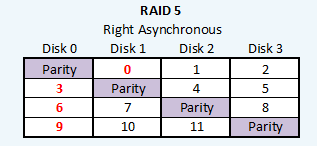
\includegraphics[scale = 1.40]{images/raid5.png}
\caption{Design of the RAID-5 system and distribution of parity blocks}
\label{overflow}
\end{figure}

So, given the disk address, c,h and s can be calculated  as:
\begin{itemize}
\item a = DiskAddress/D;

\item p = a\%(D+1) 

\item {If p is less than or equal to DiskAddress\%D then d = DiskAddress\%D  \\
	else, d = DiskAddress\%D + 1}
\item c = a/(M*K)
\item t = [ a/K ] modulo M
\item s = a modulo K
\end{itemize}

An array of all disk objects are created and read/write operations are done on them.
\begin{enumerate}
\item \textbf{Read Sector} -  Sector is read from the corresponding disk and returned back.
\item \textbf{Write Sector} - Both the requested and parity blocks are first read. XOR of bits of old data, the new data and the parity block is written back to parity block. New data is written to the corresponding sector. Total 2 reads and 2 writes are performed.
\end{enumerate}

After any operation, one pending request from buffer of each disk is executed.

\subsection{Request Buffer and Elevator algorithm \\ (diskRequestHandler.cpp \& diskRequestHandler.h)}
\paragraph{}

This contains a class which places the requests into a request buffer and processes it using the elevator algorithm. A data-structure for every request is created which also stores the time-stamp of the request.

These requests are stored in the set data structure provided by the STL of C++. This is basically a balanced binary tree structure and serves operation like search, insert and delete in time logarithmic to the size of the set i.e. the number of requests buffered in the set.

Upon serving the requests for a particular cylinder, the request structure is deleted and the arm will now move to the next closest request in the direction of movement. This request will be obtained by iterating over the tree data structure. The first element of a tree is always the leftmost one. The next element after an element is the first element of its right subtree. If the element does not have a right child, the next element is the element's first right ancestor. If the element has neither a right child nor a right ancestor, it is the rightmost element and it's last in iteration. 

In this manner the requests will be served until the start/end of the tree has been reached (depending on the direction of the movement). When the start/end has been reached, the direction of iteration will be reversed.

\begin{figure}[ht!]
\center
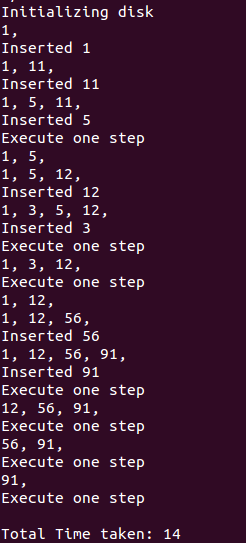
\includegraphics[scale = 0.7]{images/elevatorDemo.png}
\caption{Elevator Algorithm in action}
\label{overflow}
\end{figure}

While the traversal is being done, various statistics are being gathered like the number of times the cylinder switch is happening (i.e. the arm movement), the rotational latency incurred and the track switch. Printing the requests in the buffer is also supported which shows how the requests are being processed and queued up.

\section{Analysis of data and statistics \\ (main.cpp \& testData.py)}
\paragraph{}
For computing the statistics data, first all the file pages are written. Then requests are randomly generated which access disks to read or write data. Global flags cacheEffect and elevatorEffect are kept which can be changed true/false and all classes works correspondingly.

\subsection{Effect of elevator algorithm}
\paragraph{}

\begin{figure}[ht!]
\center
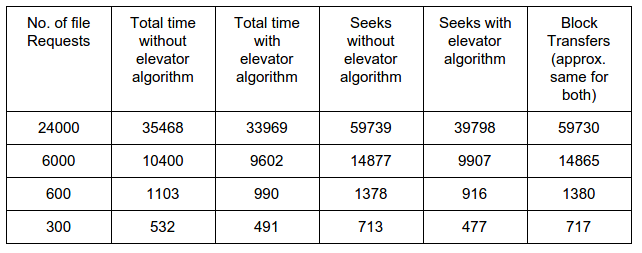
\includegraphics[scale = 0.70]{images/table1.png}
\caption{Statistics of time taken, seeks and block transfers by varying no. request}
\label{overflow}
\end{figure}



The plot of number of seeks required vs no. of requests are plotted in the below graph. The blue plot describes seeks with the elevator algorithm and the red one without elevator.

\begin{figure}[ht!]
\center
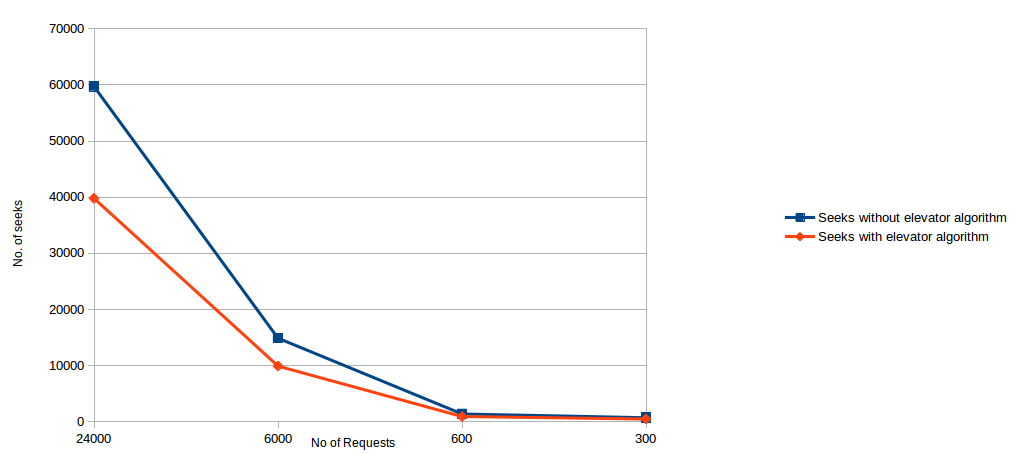
\includegraphics[scale = 0.65]{images/img0.png}
\caption{Seeks vs no. of requests}
\label{overflow}
\end{figure}


From the above graph, we can see that for a given number of requests, Number of seeks without elevator algorithm is greater than that without it. In elevator algorithm, requests are sorted in order of cylinder number.Therefore requests on same cylinder can be completed without making any seek. Thus extra seek time is avoided using elevator algorithm.



\begin{figure}[ht!]
\center
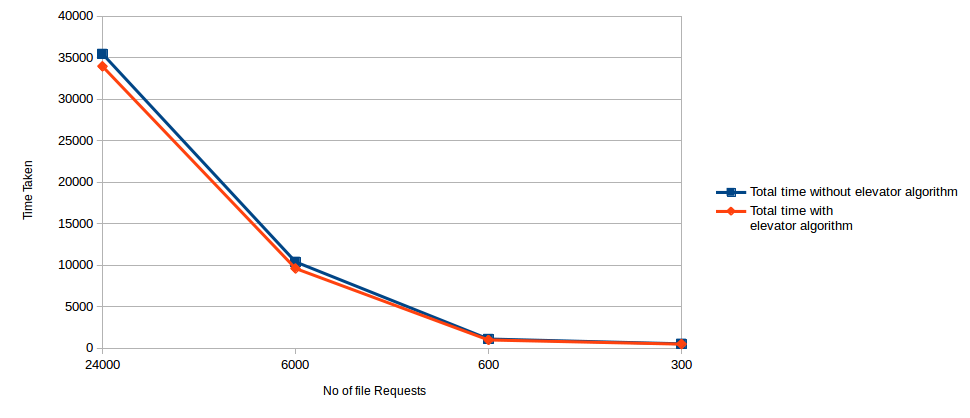
\includegraphics[scale = 0.63]{images/img1.png} 
\caption{Time taken vs. no. of requests}
\label{overflow}
\end{figure}

From the graph given below, we can see for a given number of requests total time taken with elevator algorithm is always less than that without it. 

\subsection{Effect of caching on the disk}
\paragraph{}

\begin{figure}[ht!]
\center
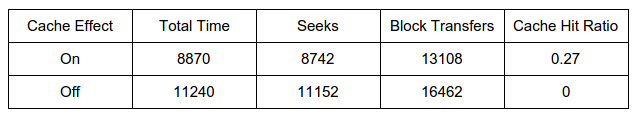
\includegraphics[scale = 0.70]{images/table2.png}
\caption{Effect of cache on no. of seeks, block transfers, total time and cache hit ratio}
\label{overflow}
\end{figure}



On switching on the cache, seeks and block transfers decreases eventually decreasing the total time. Disk addresses are accessed randomly therefore cache hit ratio is not much higher. 


\subsection{Effect of increasing the no. of disks, while keeping the total space constant}
\paragraph{}


\begin{figure}[ht!]
\center
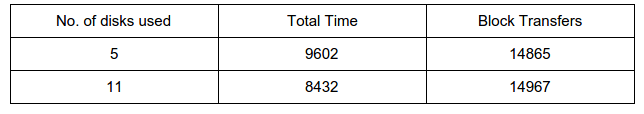
\includegraphics[scale = 0.60]{images/table3.png}
\caption{Effect of increasing the no. of disks while keeping the total }
\label{overflow}
\end{figure}


For same number of total disk size, we increased the no. of disks and found that as we increase raid level total time taken for same requests is decreased. This is due to dispersion of requests among many disks.

\subsection{Effect of increasing the cache size on no. of seeks and time taken}
\paragraph{}

\begin{figure}[ht!]
\center
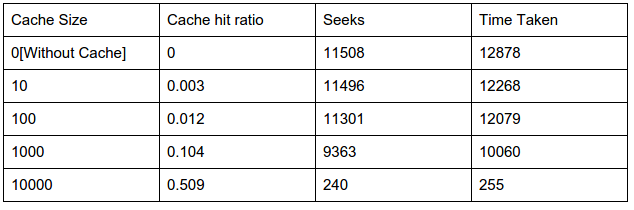
\includegraphics[scale = 0.60]{images/table4.png}
\caption{Effect of increasing the no. of disks while keeping the total }
\label{overflow}
\end{figure}


Graphs for the above table are


\begin{figure}[ht!]
\center
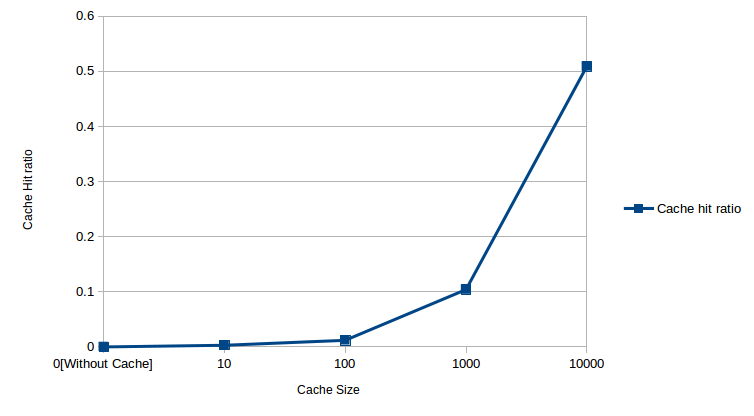
\includegraphics[scale = 0.70]{images/cache.png}
\caption{Effect on cache hit rate by increasing the cache size }
\label{overflow}
\end{figure}


We can see that the cache hit ratio(\#cache-hits/\#total-accesses) decreases as cache size increases. More pages can be stored increasing number of cache hits.


\begin{figure}[ht!]
\center
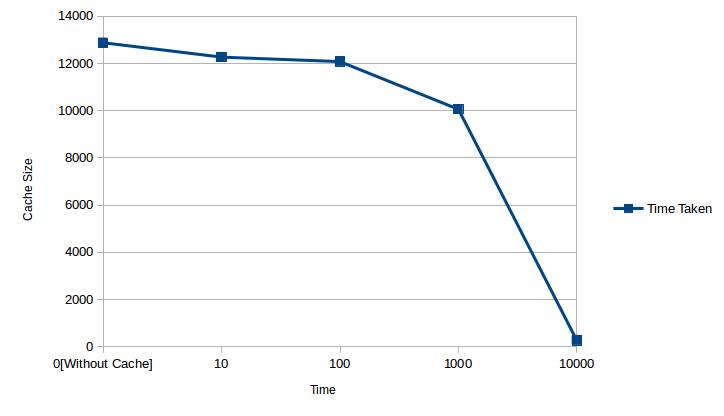
\includegraphics[scale = 0.60]{images/cache2.png}
\caption{Effect on total time by increasing the cache size}
\label{overflow}
\end{figure}

As the cache size increases, the time taken to execute reduces drastically after some time. This is because some pages are already cached which need not be written back or read from the disk. As size of cache increases more such pages can be cached.

\section{Conclusions}
\paragraph{}
In this report we talked about simulating a disk system and various aspects associated with it. It was seen that implementing RAID-5 technology demands more resources but in turn uses lesser no. of disks.
 
We learned how paging is implemented in hard disks and how pages of a file is distributed in various disks to provide an interleaved-parity RAID system. We saw and discovered the effect and importance of efficient data structures \& algorithms and caching in the implementation by various statistics.

\end{document}

